%!TeX root=../tese.tex
%("dica" para o editor de texto: este arquivo é parte de um documento maior)
% para saber mais: https://tex.stackexchange.com/q/78101

\chapter{Metodologia}

% falar sobre validação cruzada
% falar que foi em python, libs, 
% dados amostrados ao longo do tempo => não misturamos 
% validação cruzadas 
% n modelo => falar melhores

% melhorar.. só usar isso?

Nesta seção serão detalhadas as fontes dos dados utilizados no 
projeto e as estratégias de preparação e pré-processamento de 
dados. Serão descritas, ainda, as 
tecnologias utilizadas na implementação, as métricas estatísticas 
usadas para mensurar o desempenho dos modelos e o método de
 avaliação dos modelos.

\section{Dados}
\label{sec:dados}

Os algoritmos de \textit{machine learning} utilizam dados para fazer 
previsões. 
Neste trabalho, optou-se por utilizar dados de 2003 até 2019 para treinamento e 
avaliação dos modelos, em virtude da disponibilidade dos dados de consumo mensal 
de cimento. Além disso,
adotou-se granularidade
mensal e por estados de dados com o intuito de aumentar a quantidade de entradas disponíveis 
para treinamento e avaliação dos modelos.
Essa estratégia de aumento de dados, de acordo com \citet{Goodfellow-et-al-2016}, visa diminuir o risco de  
\textit{underfitting}, que acontece quando o 
modelo não é capaz de aprender com os dados e resulta em altos erros nas etapas de
treinamento e teste.


\subsection{Fontes}

O modelo utiliza dados econômicos, sociais e da construção
civil para estimar a demanda por cimento. Na tabela
\ref{tab:indicadores}, são
apresentados os dados utilizados, juntamente com a fonte, a granularidade 
e o período em que estavam disponíveis:


\begin{table}[H]
    \centering
    \caption{Indicadores utilizados no trabalho}
    \begin{tabular}{llll}
        \toprule
        Dado                   & Fonte & Período disponível & Granularidade         \\
        \midrule
        PIB a preços constantes     
                                    & IBGE\footnote{\label{portal ipea} Dado retirado do portal do Ipeadata em \url{http://www.ipeadata.gov.br/Default.aspx}}  & 1983 até 2019      & anual por estado      \\
        PIB a preços de mercado      & IBGE\footref{portal ipea}  & 1985 ate 2019      & anual por estado      \\
        PIB \textit{per capita}              & IBGE\footref{portal ipea}  & 1985 até 2019      & anual por estado      \\
        PIB da construção civil      & IBGE\footref{portal ipea}  & 1985 até 2019      & anual por estado      \\
        Desemprego                   & IBGE\footref{portal ipea}  & 1991 até 2022      & irregular \footnote{Havia dados de 1992 até 2014
        com granularidade anual e por estado. A partir de 2012, foram disponibilizados dados mensais a nível de Brasil por conta da 
        Pesquisa Nacional por Amostra de Domicílios Contínua (PNAD Contínua) realizada pelo IBGE. Neste trabalho, utilizou-se os dados anuais até 2012
        e, após 2012, os dados provenientes da PNAD Contínua.} \\
        IPCA                        & IBGE\footnote{Dado retirado do IBGE em \url{https://sidra.ibge.gov.br/tabela/1737}}  & 1981 até 2021      & mensal para o Brasil      \\
        INCC                        & FGV\footnote{Dado obtido a partir do portal da FGV em \url{https://www.debit.com.br/tabelas/tabela-completa-pdf.php?indice=incc}}   & 1980 ate 2021      & mensal para o Brasil      \\
        IGP                         & FGV\footref{portal ipea}   & 1944 até 2021      & mensal para o Brasil      \\
        Taxa Selic                  & IBGE\footnote{Dado obtido em \url{https://www.debit.com.br/tabelas/tabela-completa.php?indice=selic}}  & 1986 até 2022      & mensal para o Brasil      \\
        NFSP                        & BACEN\footref{portal ipea}  & 1991 até 2022      & mensal para o Brasil      \\
        Estoque líquido de capital fixo   & IPEA\footref{portal ipea}   & 1947 ate 2019      & anual para o Brasil      \\
        População                   & IBGE\footnote{Dado obtido do portal Base dos Dados em \url{https://basedosdados.org/dataset/br-ibge-populacao}}   & 1991 até 2021      & anual por estado      \\
        IDH                         & IBGE\footref{portal ipea}   & 1991 ate 2017      & irregular\footnote{Os indicadores de IDH (Renda, Longevidade e Educação) estão disponíveis a nível de estado da União em anos de censo do IBGE (1990, 2000, 2010). Há 
        dados, também, de 2014 a 2017 por conta da PNAD Contínua.}      \\
        Produção mensal de cimento  & SNIC\footnote{\label{cbic} Dados retirados do portal \url{http://www.cbicdados.com.br/menu/materiais-de-construcao/cimento}}  & 2003 até 2022      & mensal por estado      \\
        Valor médio do cimento\footnote{Evolução do valor médio/mediano do cimento Portland 32 em US\$/Tonelada}      & SNIC\footref{cbic}   & 1947 ate 2019      & anual para o Brasil      \\
        Consumo de cimento em ton.  & SNIC\footref{cbic} & 2003 até 2019 & mensal por estado \\
        \bottomrule
    \end{tabular}
    \label{tab:indicadores}
\end{table}
% quem sabe por a legenda no apendice

Na tabela, são utilizadas siglas 
para melhorar a legibilidade; uma descrição das abreviações utilizadas no 
trabalho pode ser encontrada no início do documento, mais especificamente na Lista de Abreviaturas.

\subsection{Preparação dos dados}

Com o intuito de direcionar a estratégia de preparação de dados,
foi realizada uma análise exploratória dos dados de 
entrada e da variável resposta. 
Na análise em questão, foi identificada uma alta taxa de variação nos atributos, sendo possível a observância de um grande número de \textit{outliers} presente nos dados.
De acordo com \citet{outliers} e \citet{tukey77}, \textit{outliers} são
observações discrepantes do restante dos dados
que podem interferir no processo de previsão. 

Um exemplo de atributo com alta variação é o PIB da contrução civil,
que apresenta desvio padrão maior que o valor médio dessa variável.
Para ilustrar a distribuição dos pontos de dados desse indicador, foi utilizado 
um gráfico \textit{boxplot} na figura \ref{fig:boxplot_pibcc}:

\begin{figure}[H]
    \centering
    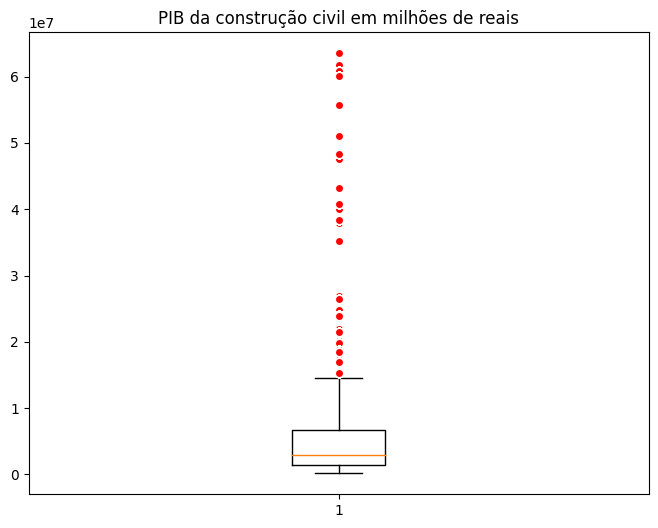
\includegraphics[width=9cm]{../figuras/graficos/boxplot-pib-cc.png}
    \caption{Gráfico \textit{boxplot} do PIB da construção civil construído a partir dos dados disponíveis no portal do IPEA, conforme descrito na tabela \ref{tab:indicadores}}
    \label{fig:boxplot_pibcc}
\end{figure}

Segundo \citet{boxplot}, o \textit{boxplot} é
uma técnica estatística utilizada para identificar visualmente padrões nos dados. 
Na figura acima, a linha em laranja corresponde à mediana\footnote{Mediana é
valor que fica no meio quando os dados estão ordenados ou a média
dos dois valores centrais se o número de pontos de dados for par.
(\cite{boxplot-stat})} 
dos dados, os limite inferior e o superior do retângulo representam
o primeiro e terceiro quartis\footnote{O primeiro quartil marca a mediana 
relativa aos valores superiores à mediana destacada na imagem. O terceiro quartil,
de maneira análoga, assinala a mediana dos valores inferiores à mediana destacada. 
Assim, entre o primeiro e terceiro quartis está contida metade
dos dados.}, respectivamente. As observações fora do intervalo dos limites 
superior e inferior, representadas com círculos vermelhos na figura, são 
\textit{outliers}. Pode-se observar, então, a alta incidência de dados discrepantes
nesse indicador.

Parte do alto volume de \textit{outliers} nos atributos se deve às diferenças
econômicas, geográficas e sociais entre os estados do Brasil. A saber, o valor 
médio do PIB da construção civil no estado 
de São Paulo é de $48.96$ milhões, enquanto em Santa Catarina é de $7.1$ milhões e 
em Roraima, de $0.4$ milhões. Aliás, ao analisar o PIB da construção civil nas 
regiões do país, há uma significativa redução no número de dados discrepantes, como é possível
pode observar na figura abaixo:

\begin{figure}[H] 
    \centering
    \begin{subfigure}{5cm}
      \centering 
      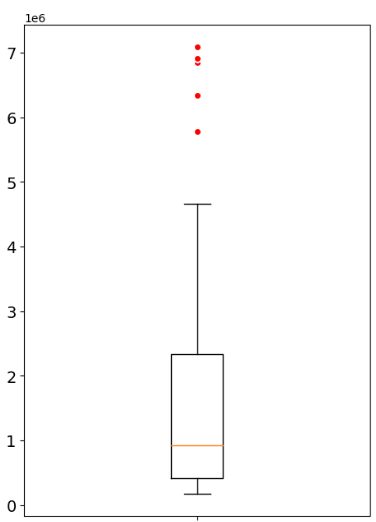
\includegraphics[width=4.5cm]{../figuras/graficos/boxplot-pib-cc-n.png}
      \caption{Região Norte}
      \label{fig:boxplot-n}
    \end{subfigure}
    \hfill 
    \begin{subfigure}{5cm}
        \centering 
        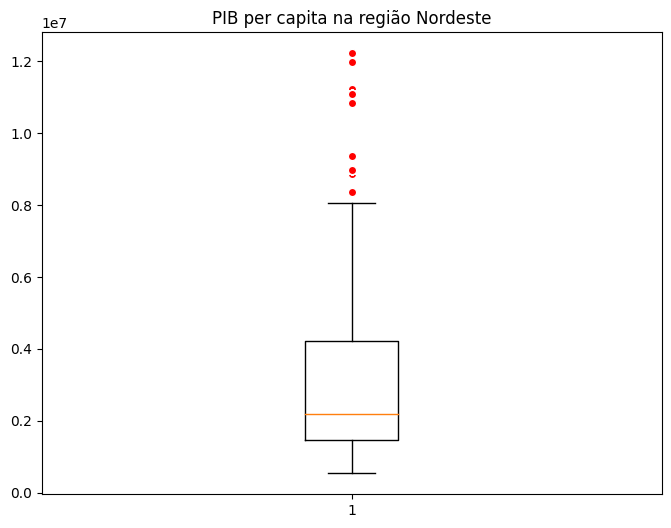
\includegraphics[width=4.5cm]{../figuras/graficos/boxplot-pib-cc-ne.png}
        \caption{Região Nordeste}
        \label{fig:boxplot-ne}
    \end{subfigure}
    \begin{subfigure}{5cm}
        \centering 
        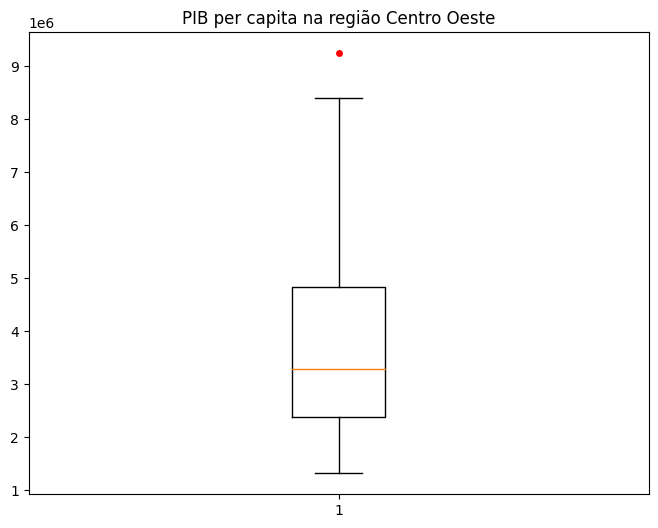
\includegraphics[width=4.5cm]{../figuras/graficos/boxplot-pib-cc-co.png}
        \caption{Região Centro Oeste}
        \label{fig:boxplot-co}
    \end{subfigure}
    \begin{subfigure}{5cm}
        \centering 
        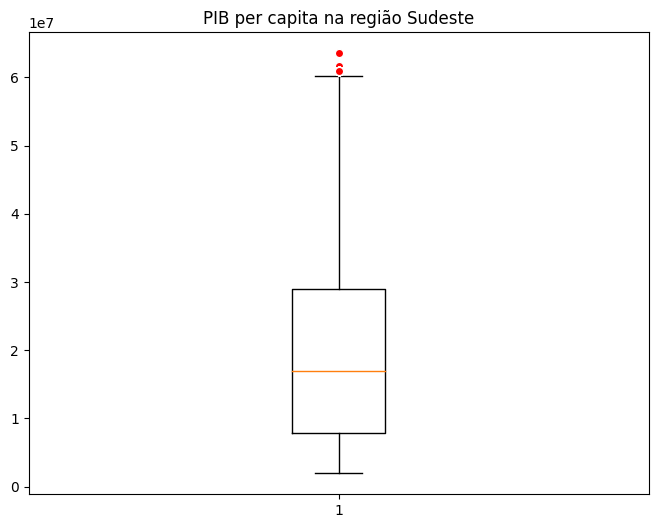
\includegraphics[width=4.3cm]{../figuras/graficos/boxplot-pib-cc-se.png}
        \caption{Região Sudeste}
        \label{fig:boxplot-se}
    \end{subfigure}
    \begin{subfigure}{5cm}
        \centering 
        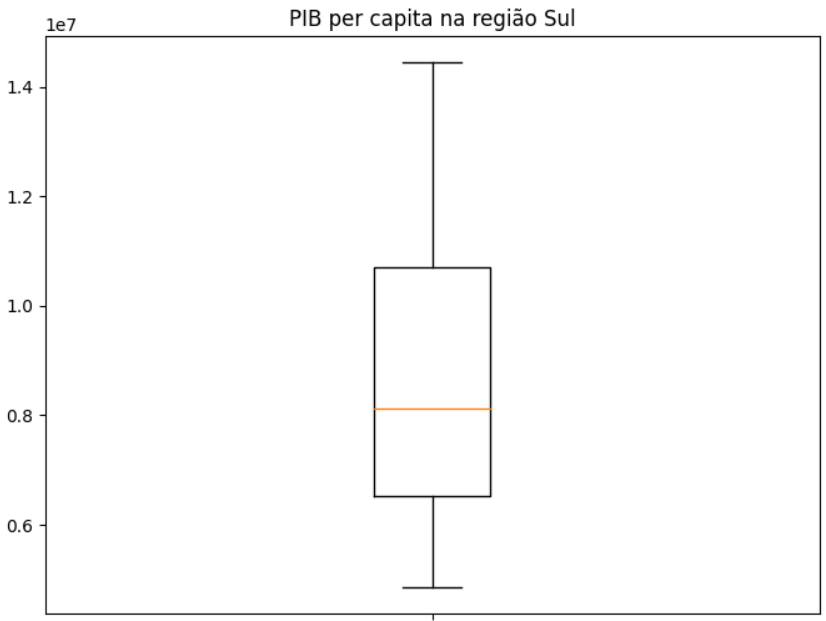
\includegraphics[width=4.5cm]{../figuras/graficos/boxplot-pib-cc-s.png}
        \caption{Região Sul}
        \label{fig:boxplot-s}
    \end{subfigure}
    \caption{Comparação dos gráficos \textit{boxplot} entre as regiões}
  \end{figure}

Além disso, a correlação entre as variáveis de entrada foi analisada com o auxílio 
de uma matriz de correlação, o que gerou a identificação de uma 
alta correlação entre os indicadores do PIB do estado, o PIB da construção
civil e o tamanho da população. Por fim, também foi observada a correlação entre os três indicadores
de IDH (longevidade, saúde e renda) e entre o preço do saco de cimento e o preço do kilograma, como pode-se
validar na figura \ref{fig:matriz-corr}:

\begin{figure}[H]
    \centering
    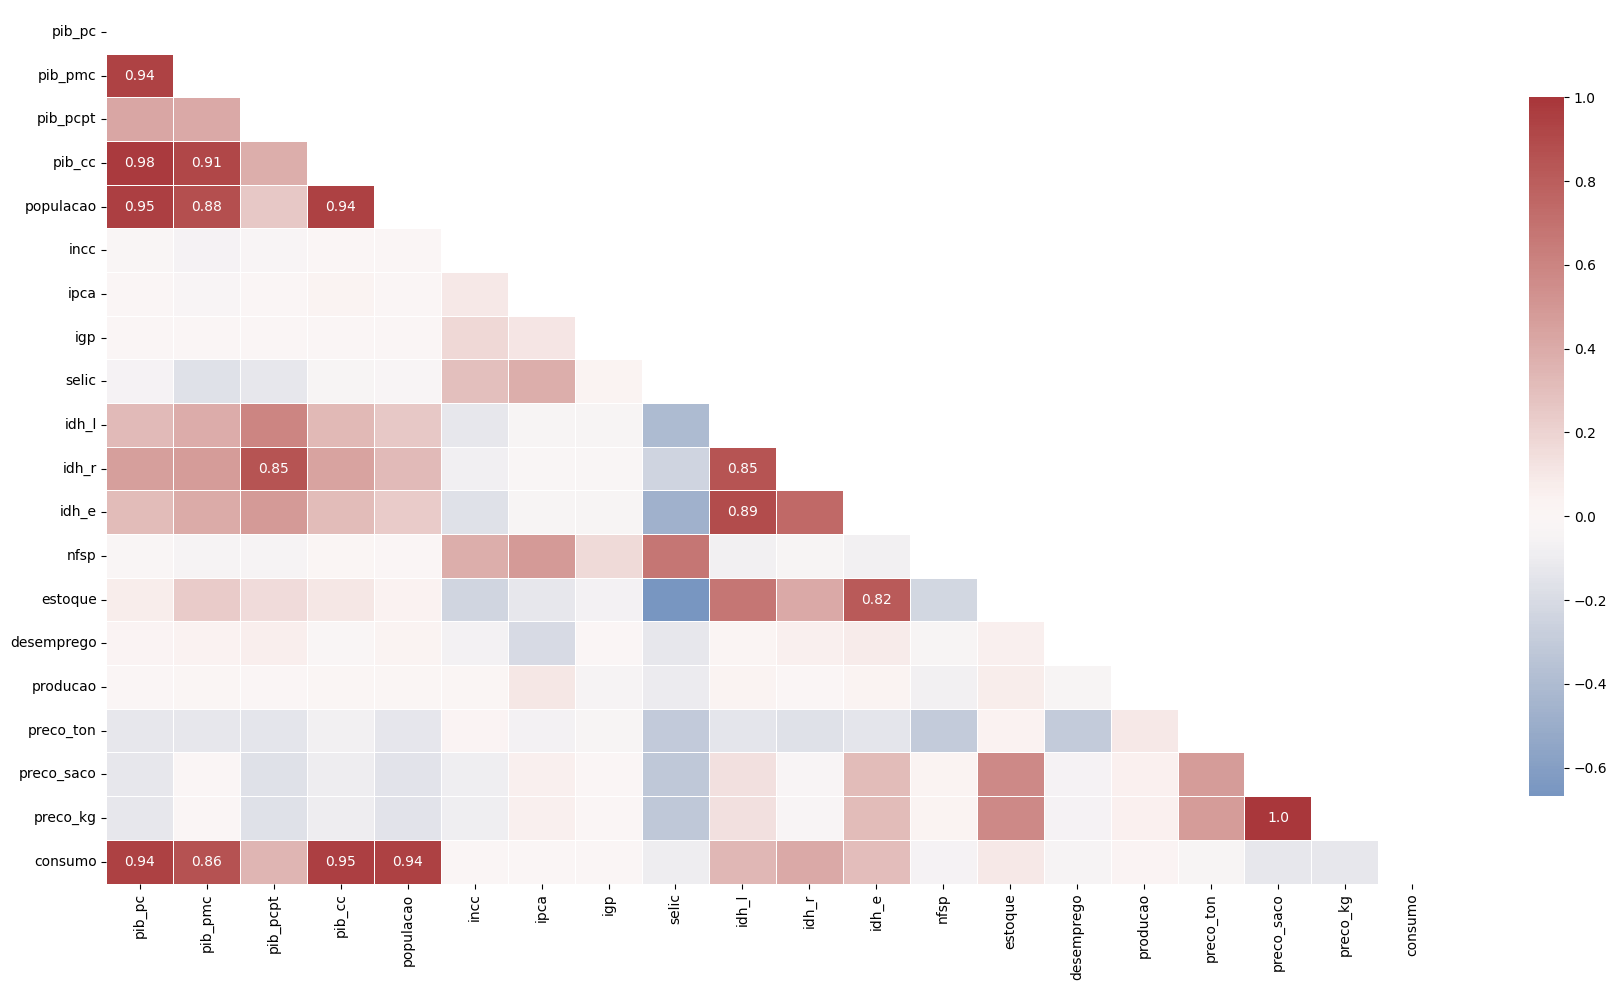
\includegraphics[width=13cm]{../figuras/graficos/matriz-corr.png}
    \caption{Matriz de correlação}
    \label{fig:matriz-corr}
\end{figure}

Foram adotadas estratégias para garantir que os dados estivessem na granularidade\footnote{A granularidade original dos dados está na tabela \ref{tab:indicadores}.}
mensal e por estado. Caso os indicadores apresentassem granularidade anual, o valor de
cada medição seria dividido por 12 de modo a obter a média mensal utilizada em 
todos os meses do ano correspondente. Caso a granularidade
fosse a nível de Brasil, o valor apresentado seria repetido para todos os 
estados no mês e ano correspondentes. As exceções foram os 
indicadores de IDH, por apresentarem valores apenas em anos específicos, conforme 
detalhado na tabela \ref{tab:indicadores}, quando não havia dados para um 
determinado ano, o valor da última medição foi repetido.

Também foi necessário lidar com dados faltantes e, para isso, o método utilizado foi
repetir o último valor disponível nos dados de entrada para
preencher a ocorrência faltante. Contudo, para a produção mensal de cimento e para os 
indicadores de evolução do preço do cimento, foi utilizado um valor não 
presente no intervalo dos dados de entrada (-1) para marcar as ocorrências 
faltantes como nulo, uma vez que essas variáveis não apresentavam 
valores mais antigos.

Além disso, garantiu-se que a previsão
 utilizasse dados dos meses anteriores e não do mês alvo da
previsão, uma vez que o objetivo do projeto é prever a demanda
por cimento em um mês a partir dos dados disponíveis no mês anterior.
Por isso, nos dados com granularidade anual, foi realizado um 
deslocamento de modo a associar as entradas de um ano ao consumo no 
ano seguinte. Nos dados mensais, analogamente, deslocaram-se as entradas 
para associá-las ao consumo no mês seguinte.

Por fim, o estado correspondente à medição foi usado como dado de entrada. 
Como os modelos de inteligência artificial aceitam apenas caracteres numéricos,
utilizou-se o método de codificação \textit{one hot} para criar 27 colunas, uma
para cada estado, nas quais o valor é um quando a linha possui dados daquele estado 
e é zero em caso contrário.


\subsection{Pré-processamento de dados}
\label{sec:norm_dados}

Foram utilizadas técnicas de pré-processamento de dados 
com o intuito de garantir que as variáveis de entrada 
estivessem na mesma escala. Esse processo tem a finalidade de permitir a comparação 
entre variáveis com diferentes unidades e melhorar o funcionamento dos 
algorimos de \textit{machine learning}, uma vez que se as \textit{features} estiverem em escalas diferentes,
alguns pesos podem ser atualizados mais rápidos que outros, segundo \citet{Raschka}.
Tendo o que se disse em mente, foram testadas no presente trabalho: normalização, 
\textit{min-max scaler} e \textit{power transformer}.

\subsubsection{Normalização}

A normalização garante que as variáveis de entrada estejam em uma 
escala com as propriedades de uma distribuição normal: média ($\mu$)
igual a zero e variância ($\sigma$) igual a um. Dessa forma, a operação 
realizada para aplicar o processo em uma entrada $x$ é:

\begin{equation}
  x_{norm} = \frac{x - \mu}{\sigma}
\end{equation}

\subsubsection{\textit{Min-Max scaler}}

De acordo com \citet{Raschka}, o \textit{min-max scaler} é uma 
abordagem alternativa à normalização 
e transforma os dados de modo que a 
escala tenha um intervalo definido, em geral, entre
0 e 1. A operação aplicada em uma entrada $x$ para é:

\begin{equation}
  x_{norm} = \frac{x - x_{min}}{x_{max} - x_{min}}
\end{equation}

Sendo $x_{norm}$ a versão normalizada da entrada $x$, e $x_{min}$ e $x_{max}$
os valores mínimo e máximo assumidos por $x$. 

\subsubsection{\textit{Power transformer}}

O \textit{power transformer} é outra alternativa para aproximar os dados 
de uma distribuição normal, esse método visa estabilizar a variância e 
diminuir a assimetria dos dados por meio da aplicação da 
transformação de \citet{yeo} nas entradas. 


\section{Avaliação de performance}

Para comparar a eficiência dos modelos, mede-se os erros de 
cada previsão, ou seja, a distância entre o valor previsto 
pelo algoritmo e o valor do dado real. Neste trabalho, 
utilizou-se as seguintes métricas estatísticas para 
mensurar o desempenho: \textit{mean absolute error} (MAE),
\textit{root mean square  error} (RMSE) e \textit{mean 
absolute percentage error} (MAPE). Além disso, foi utilizada
a variação percentual ($\Delta$) para avaliar se o modelo tende 
a subestimar ou superestimar o valor previsto.

\subsection{\textit{Mean absolute error} (MAE)}

De acordo com \citet{forecast-evaluation-ds}, a
\textit{mean absolute error} (MAE)
mede o erro absoluto de cada previsão. Seja $\hat{y_i}$ o valor previsto pelo 
modelo e $y_i$ o valor real, a fórmula da MAE é dada por:

\begin{equation}
    MAE = \frac{\sum_{i=1}^n |\hat{y}_i - y_i|}{n}
\end{equation}

Essa métrica não leva em consideração a proporção do erro em relação ao valor
real, apenas o valor absoluto da diferença, dessa forma não expressa a ordem de
grandeza do erro em relação ao valor real.

\subsection{\textit{Root mean squared error} (RMSE)}

A RMSE, sigla para \textit{root mean squared  error}, é uma métrica de erro
semelhante à MAE. Sendo $\hat{y_i}$ o valor previsto pelo 
modelo para um \textit{output} $y_i$, a fórmula da RMSE é dada por: 

\begin{equation}
    RMSE = \sqrt{\frac{\sum_{i=1}^n (\hat{y}_i - y_i)^2}{n}}
\end{equation}

A RMSE é influenciada por erros mais significativos, dessa forma, é mais 
sensível a \textit{outliers} que a MAE, segundo \citet{forecast-evaluation-ds}. 

\subsection{\textit{Mean absolute percentage error} (MAPE)}

Foi utilizada também a \textit{mean absolute
percentage error}, para mensurar a magnitude do erro em 
relação ao tamanho das medições, a MAPE calcula a proporção 
do erro em relação ao valor que o modelo tentou prever. Sendo $\hat{y_i}$ 
o valor previsto pelo 
modelo para um \textit{output} $y_i$, a fórmula da MAPE é dada por: 

\begin{equation}
    MAPE=\sum_{t=1}^n\left|\frac{y_t-\hat{y}_t}{y_t}\right|
\end{equation}

A MAPE proporciona uma visão do tamanho do erro em relação ao valor que se 
deseja prever.

\subsection{Variação percentual}

A variação percentual, $\Delta$, é utilizada para mensurar se o 
modelo apresenta tendência de subestimar ou superestimar a variável. 
Sendo $\hat{y_i}$ o valor previsto pelo 
modelo para um \textit{output} $y_i$, a fórmula da variação percentual
$\Delta$ é dada por:

\begin{equation}
    \Delta = \frac{\hat{y_i} - y_i}{y_i}
\end{equation}

\section{Avaliação do desempenho do modelo}

Neste trabalho, separou-se a massa de dados em conjunto de treino com 85\% 
das entradas e de teste com 15\% do conjunto, a metodologia empregada teve como objetivo avaliar
a capacidade de generalização do modelo e, por medir o desempenho em dados 
desconhecidos pelo modelo, também permite avaliar a ocorrência de \textit{overfitting}\footnote{
O \textit{overfitting} ocorre quando um modelo tem baixa capacidade de generalização, 
então, apesar de apresentar baixa taxa de erro nos dados de treino, apresenta 
desempenho ruim em dados não conhecidos.}. Levando isso em conta, não foi utilizado embaralhamento de dados, 
logo, os modelos foram treinados com dados de janeiro de 2003 até junho de 2017,
e testados com dados de julho de 2017 até dezembro de 2019.

\section{Tecnologias utilizadas}

Neste projeto\footnote{Os códigos utilizados no projeto estão disponíveis em \url{https://github.com/LeiteJu/TCC}.} foi utilizada a linguagem Python e  o ambiente de desenvolvimento interativo fornecido pelo Jupyter Notebook\footnote{O projeto Jupyter, cujo nome é originado da junção do nome das linguagens Julia, Python e R, provê um 
ambiente de desenvolvimento interativo baseado em \textit{web}. Nos \textit{notebooks}, é possível executar células de código 
em várias linguagens, além de inserir células de Markdown para auxiliar na documentação, explicação e organização do código. Essas informações foram 
retiradas de \url{https://jupyter-notebook.readthedocs.io/en/stable/notebook.html}.}.
Foram utilizadas as bibliotecas Pandas\footnote{A Pandas é uma ferramenta \textit{open source} para análise e manipulação de dados em Python, informação retirada da documentação oficial em \url{https://pandas.pydata.org/about/index.html}.} e NumPy\footnote{
Numpy é um pacote que provê operações matemáticas em vetores, segundo a documentação \url{https://numpy.org/doc/stable/}
} para realizar a preparação dos dados,
além da TensorFlow\footnote{TensorFlow é uma biblioteca que permite a criação de modelos de aprendizado de máquina, informação retirada de \url{https://www.tensorflow.org/learn?hl=pt-br}.} e Scikit-learn com o intuito de treinar e avaliar os modelos.
A maior parte dos gráficos foi gerada por meio das bibliotecas 
Seaborn e Matplotlib, contudo, alguns foram contruídos por meio da plataforma
Microsoft Excel.
